\chapter{SCRUM Dokumentation}
\label{chapter:scrum-documentation}
Grundet projektgruppens størrelse og sammensætning er det valgt at lave en meget tilpasset version af \emph{SCRUM}. Dermed er bl.a. \emph{retrospective} og \emph{review} slået sammen under "Udførelse". 
Dette er også gjort, fordi der ikke er en \emph{Product Owner}. I \Cref{sec:conclusion_summary} konkluderes der på selve \emph{SCRUM}-processen i projektet.

\section{Sprint 1}
\label{sec:sprint-1}
\subsection{Planlægning}
\label{subsec:sprint-1-plan}
\begin{itemize}
    \item \textbf{Start:} 22-04-2024
    \item \textbf{Slut:} 26-04-2024
    \item \textbf{Mål:} Oprettelse af projektet, yderligere design, konfiguration af \emph{Razor Pages} og \emph{EF}, oprettelse af modeller, oprettelse af dokumentation.
    \item \textbf{User Stories fuldført:} US-001, US-002, US-003, US-004, US-005, US-006, US-007, US-008, US-009
    \item \textbf{Story Points:} 27
\end{itemize}

\subsection{Udførelse}
\label{subsec:sprint-1-udforelse}
Sprintet var præget af, at der var mange forskellige opgaver, der skulle påbegyndes, og mange ideer. 
Derudover skulle mange styringsværktøjer som \emph{Trello}, \emph{GitHub}, \emph{Visual Studio} og \emph{SQL Server} sættes op og konfigureres. 
Særligt \emph{Trello} var en udfordring, da der ikke var en god måde at skabe et detaljeret overblik over fx \emph{Tasks} eller udtrække data på. 
Derfor blev der brugt tid på at lave en \emph{WinForm}-applikation, der kunne trække data ud af \emph{Trello} - som kun kunne udtrækkes i \emph{JSON}-format - og skrive det til \emph{Markdown}, \emph{LaTeX} og \emph{CSV} med henblik på at kunne importere det igen. 
\emph{TrelloConverter} kan findes på \emph{GitHub} \cite{trello-converter}. 
Alle \emph{story points} blev dog nået til tiden, omend en del af selve designet og \emph{bootstrap} blev nedprioriteret, da det ikke var essentielt for at kunne komme i gang med projektet.

\section{Sprint 2}
\label{sec:sprint-2}
\subsection{Planlægning}
\label{subsec:sprint-2-plan}
\begin{itemize}
    \item \textbf{Start:} 29-04-2024
    \item \textbf{Slut:} 03-05-2024
    \item \textbf{Mål:} Oprettelse af produkter, oprettelse af kunder, oprettelse af ordrer, oprettelse af bestillinger, oprettelse af betalinger, oprettelse af statistikker, oprettelse af dokumentation.
    \item \textbf{User Stories fuldført:} US-010, US-011, US-012, US-013, US-014, US-015, US-016, US-017, US-018
    \item \textbf{Story Points:} 28
\end{itemize}

\subsection{Udførelse}
\label{subsec:sprint-2-udforelse}
Sprintet var meget fokuseret på implementering af modeller og \emph{controllers} samt at få \emph{EF} konfigureret. 
Der blev brugt meget tid på at anvende \emph{HttpContextAccessor}, da det var nødvendigt for at kunne gøre \emph{HTTP} mere \emph{stateful} og dermed kunne gemme oplysninger hos klienten.

\section{Sprint 3}
\label{sec:sprint-3}
\subsection{Planlægning}
\label{subsec:sprint-3-plan}
\begin{itemize}
    \item \textbf{Start:} 06-05-2024
    \item \textbf{Slut:} 10-05-2024
    \item \textbf{Mål:} Oprettelse af \emph{IdentityCore}, oprettelse af brugere, oprettelse af roller, oprettelse af \emph{claims}, oprettelse af dokumentation.
    \item \textbf{User Stories fuldført:} US-019, US-020, US-021, US-022, US-023, US-024, US-025, US-026, US-027
    \item \textbf{Story Points:} 28
\end{itemize}

\subsection{Udførelse}
\label{subsec:sprint-3-udforelse}
Meget af tiden gik med at få \emph{IdentityCore} til at fungere, da det var nødvendigt for at kunne lave en brugeroplevelse, der var tilpasset de forskellige roller.
Det var især den bagvedliggende dokumentation, der var udfordrende, da der var mange forskellige måder at gøre tingene på og mange forskellige måder at konfigurere det på.
Der blev brugt meget tid på at overveje og afprøve forskellige løsninger, da det var nødvendigt at have en løsning, der kunne skaleres og vedligeholdes.

\section{Sprint 4}
\label{sec:sprint-4}
\subsection{Planlægning}
\label{subsec:sprint-4-plan}
\begin{itemize}
    \item \textbf{Start:} 13-05-2024
    \item \textbf{Slut:} 17-05-2024
    \item \textbf{Mål:} Oprettelse af brugergrænseflade, oprettelse af brugeroplevelse, oprettelse af dokumentation.
    \item \textbf{User Stories fuldført:} US-028, US-029, US-030, US-031, US-032
    \item \textbf{Story Points:} 28
\end{itemize}

\subsection{Udførelse}
\label{subsec:sprint-4-udforelse}
Meget af tiden gik med at få brugergrænsefladen til at fungere, da det var nødvendigt for at kunne lave en brugeroplevelse, der var tilpasset de forskellige roller.
Med dette tænkes især på kunders interaktion med systemet og hvordan data blev håndteret. 
Dette kan ses bl.a. på \emph{Index}-siden med billedekarusel og på \emph{Katalog} (\emph{CustomerProducts/Index}), hvor der er forskellige muligheder for at filtrere og sortere data.

\section{Sprint 5}
\label{sec:sprint-5}
\subsection{Planlægning}
\label{subsec:sprint-5-plan}
\begin{itemize}
    \item \textbf{Start:} 20-05-2024
    \item \textbf{Slut:} 24-05-2024
    \item \textbf{Mål:} Oprettelse af statistikker, oprettelse af dokumentation.
    \item \textbf{User Stories fuldført:} US-033, US-034, US-035, US-036, US-037
    \item \textbf{Story Points:} 28
\end{itemize}

\subsection{Udførelse}
\label{subsec:sprint-5-udforelse}
Meget af tiden gik med at få analyse og dataudtræk til at fungere, da det var nødvendigt for at kunne give nogle solide data til butikken, så de kunne se, hvordan deres forretning gik.
Det tog tid at genopfriske de nødvendige kompetencer indenfor \emph{JavaScript}, da det var nødvendigt for at kunne anvende \emph{Chart.js} og få det til at fungere sammen med \emph{Razor Pages}.
Der blev også implementeret en email-service gennem \emph{MailKit}, så butikken automatisk kunne sende en email til kunden, når de havde afgivet en ordre eller bekræftet oprettelse.

\section{Sprint 6}
\label{sec:sprint-6}
\subsection{Planlægning}
\label{subsec:sprint-6-plan}
\begin{itemize}
    \item \textbf{Start:} 27-05-2024
    \item \textbf{Slut:} 30-05-2024
    \item \textbf{Mål:} Oprettelse af dokumentation, oprettelse af test, oprettelse af testdata, oprettelse af testcases.
    \item \textbf{User Stories fuldført:} US-038, US-039, US-040, US-041, US-042
    \item \textbf{Story Points:} 8
\end{itemize}

\subsection{Udførelse}
\label{subsec:sprint-6-udforelse}
Der var nogle indsatsområder, der skulle færdiggøres, såsom dokumentation og test, samt tid brugt på at få testdata til at fungere, da det var nødvendigt for at kunne teste systemet.
Der blev også brugt tid på at deployere systemet, så det kunne køre på et webhotel og dermed kunne ses i et realistisk miljø. 
\emph{Simply.com} blev valgt som webhotel, da det var billigt og nemt at konfigurere. 
I skrivende stund er projektet dog ikke deployeret, da der er problemer med at få \emph{.NET 8} til at køre på webhotellet. Projektet er dog testet lokalt og fungerer som forventet.

\section{Burndown Chart}
\label{sec:burndown-chart}
\begin{figure}[H]
    \centering
    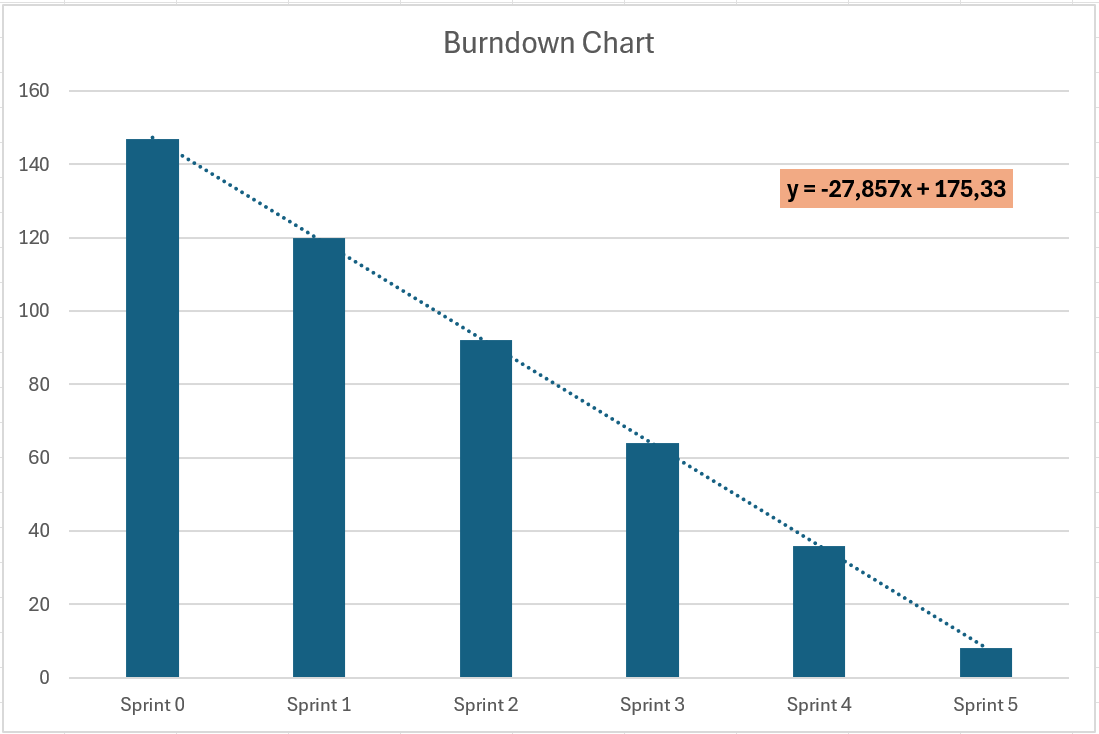
\includegraphics[width=0.8\textwidth]{figures/scrum/burndown-chart.png}
    \caption{Burndown Chart}
    \label{fig:burndown-chart}
\end{figure}

Alle \emph{sprints} blev gennemført til tiden, og alle \emph{user stories} blev gennemført til tiden. 
Der var dog en del af designet og \emph{bootstrap}, der blev nedprioriteret eller skubbet til senere \emph{sprints}, da det ikke var essentielt for den videre funktionalitet. 
Dette kan ses på \emph{Burndown Chartet} \cref{fig:burndown-chart}, hvor det er de sidste to "idé" \emph{user stories}, der ikke er blevet gennemført.
\emph{Burndown Chartet} giver en hældningskoefficient på -27,8, hvilket svarer til de ca. 28 \emph{story points}, som hvert \emph{sprint} i gennemsnit var estimeret til.
